%&tex
\documentclass[12pt]{article}

\usepackage[a4paper,margin=1in]{geometry}
\usepackage{amsmath,amssymb}

\usepackage{graphicx}
\graphicspath{{""}}

\usepackage{cleveref}
\usepackage{subcaption}

\title{Rankine Semi-infinite Body computation}
\author{Ramkumar}

\begin{document}

\maketitle

\section{Problem Definition}
In this work, Rankine semi-infinite body is computed using potential flow theory.
The code was made as a custom application in OpenFOAM v2206 and the postprocessing
is done using ParaView. The main aim of the work is to introduce the OpenFOAM
programming powers to the users.

\section{Governing equations}\label{eqnSection}
In this work, the potential flow equation containing a Uniform flow and a source
positioned appropriately to form the semi-infinite body. The main equation that
is used to compute streamfunction \(\psi\) is given below, Equation \ref{psiEqn}.


\begin{align}
	\psi = V_{\infty} \cdot r \cdot sin(\theta) + \frac{\Lambda}{2\pi}\theta \label{psiEqn}
\end{align}

The corresponding velocities in polar coordinates is given at Equations \ref{eqnVr}
and \ref{eqnVtheta} below.


\begin{align}
	V_r & = \frac{1}{r}\frac{\partial \phi}{\partial \theta} = V_{\infty} \cdot cos(\theta) + \frac{\Lambda}{2\pi r} \label{eqnVr}\\
	V_{\theta} & = -\frac{\partial \phi}{\partial r} = - V_{\infty} \cdot sin(\theta) \label{eqnVtheta}
\end{align}\\

A rectangular mesh was made using \emph{blockMesh} utility in OpenFOAM and the cell
centers in the mesh were used as the computation points for streamfunction \(\phi\) and
other variables. The radial distance \(r\) and azimuthal distance \(\theta\) are
calculated using the Equations \ref{eqnR} and \ref{eqnTheta}, respectively.

\begin{align}
	r & = \sqrt{\Delta x^2 + \Delta y^2} \label{eqnR} \\
	\theta & = arctan2( \Delta y, \Delta x) \label{eqnTheta}
\end{align}\\

The transformation equations used to convert polar velocities to cartesian ones
is given at Equations \ref{eqnU} and \ref{eqnV}.

\begin{align}
	U_x & = V_r \cdot cos(\theta) - r \cdot V_{\theta} \cdot sin(\theta) \label{eqnU} \\
	U_y & = V_r \cdot sin(\theta) + r \cdot V_{\theta} \cdot cos(\theta) \label{eqnV}
\end{align}

\section{Computation Methodology}
The steps followed in OpenFOAM to generate the semi-infinite body are given below.


\begin{enumerate}
	\item a new custom application was made in OpenFOAM v2206 and named as \emph{semiInfiniteBody} using command \emph{foamNewApp appName}.
	\item totally 6 new volScalarFields and 1 volVectorField were created to store the corresponding fields computed using the equations mentioned in the Section \ref{eqnSection}.
	\item a loop over cells is created using which the field values for each cell is computed and then at the end of loop the solution fields will be writen to the \emph{0} folder in the case directory.
\end{enumerate}

The result obtained using the OpenFOAM code is shown as a contour with streamlines that were made using \emph{ParaView}, in \Cref{fig:contour}.

\begin{figure}
	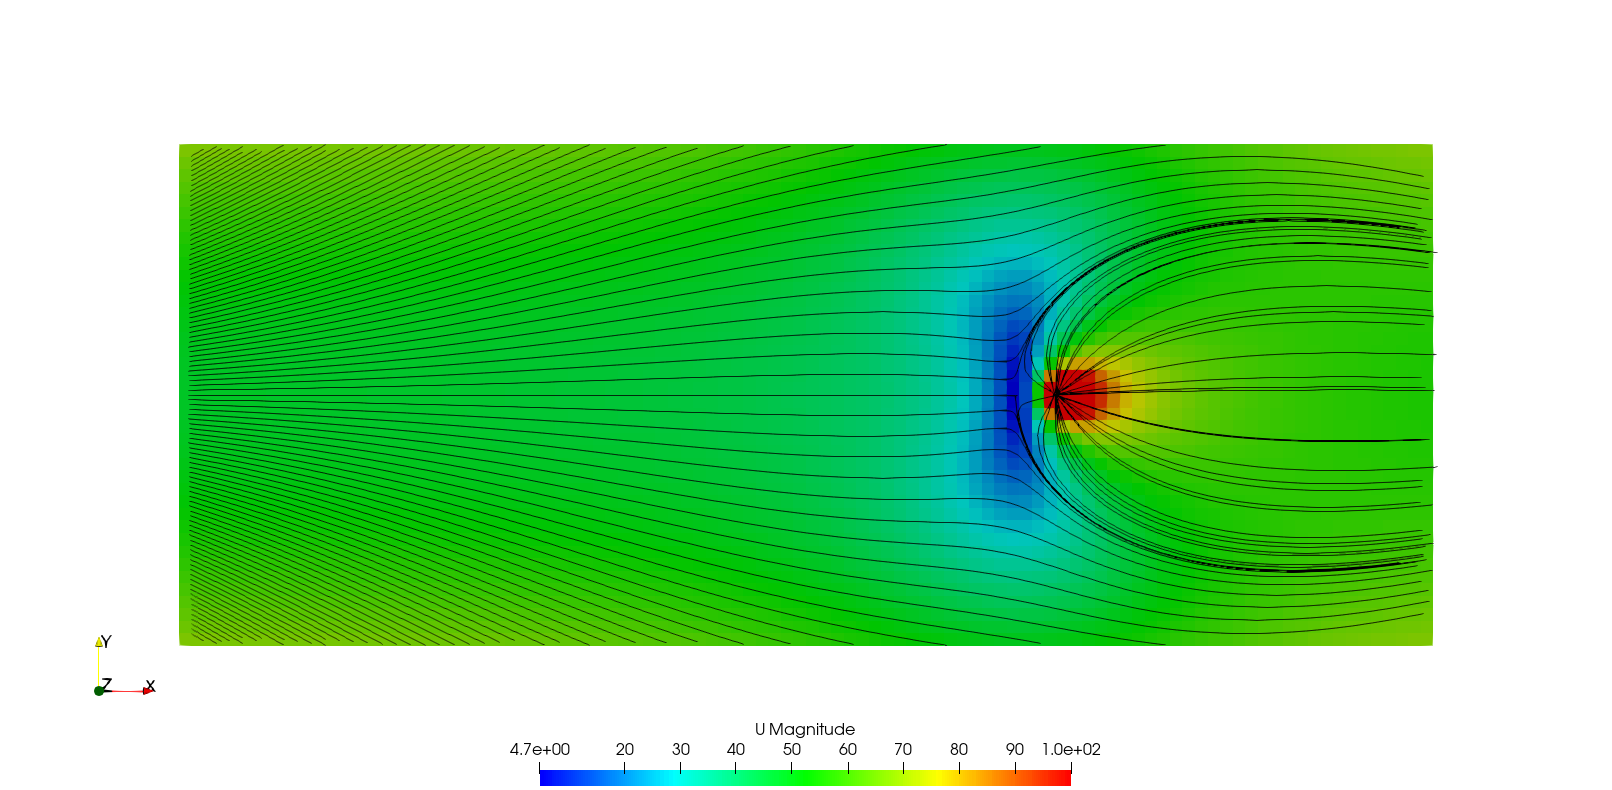
\includegraphics[scale=0.3]{streamlines.png}
	\caption{streamlines contour of semi-infinite body}
	\label{fig:contour}
\end{figure}

\section{Instructions}
The instruction to generate/execute the files present in this work is given below.

\begin{enumerate}
	\item copy the contents of this entire root folder named \emph{01\_RankineSemiInfiniteBody} to a new directory.
	\item go into the subfolder named \emph{03\_OpenFOAMCode} which contains another sub-subfolder named \emph{semiInfiniteBody}, go into that using the terminal which is enabled with OpenFOAM environment.
	\item in the terminal, type \emph{wclean} and press enter, to clean any previous compilation files. Then type \emph{wmake} and press enter, this will compile the application.
	\item after compilation, cd to the directory named \emph{02\_testCase} and execute the command named \emph{semiInfiniteBody}. this should compute the field values and store them in the \emph{0} folder.
	\item after computation, use \emph{ParaView} for visualization of results.
\end{enumerate}

\end{document}
